\documentclass[acmtog]{acmart}
\usepackage{graphicx}
\usepackage{subfigure}
\usepackage{natbib}
\usepackage{listings}
\usepackage{bm}
\usepackage{fancyhdr}
\pagestyle{empty}

\definecolor{blve}{rgb}{0.3372549 , 0.61176471, 0.83921569}
\definecolor{gr33n}{rgb}{0.29019608, 0.7372549, 0.64705882}
\makeatletter
\lst@InstallKeywords k{class}{classstyle}\slshape{classstyle}{}ld
\makeatother
\lstset{language=C++,
	basicstyle=\ttfamily,
	keywordstyle=\color{blve}\ttfamily,
	stringstyle=\color{red}\ttfamily,
	commentstyle=\color{magenta}\ttfamily,
	morecomment=[l][\color{magenta}]{\#},
	classstyle = \bfseries\color{gr33n}, 
	tabsize=2
}
\lstset{basicstyle=\ttfamily}

% Title portion
\title{Final Project:\\ {Photon Mapping}}

\author{
Group Number:\quad 5 \\
Member 1:\quad Chunhao Bi\\
Member 2:\quad Hongdi Yang\\
Member 3:\quad Mutian Li
}

% Document starts
\begin{document}
\maketitle

\vspace*{2 ex}

\section{Introduction}
	This is the final project of CS171.01. 
	In this project, the photon mapping method for rendering is introduced, and some comparisons are carried out.
\section{Algorithm}
	\subsection{Photon mapping}
		The standard photon mapping includes two passes. 
		The first is to generate photons from all light sources, and the photons will bounce between objects and stops when meeting terminate conditions.
		The photon tracing is similar to path tracing, and the photons are stored in a tree for later use.
		The second pass is ray tracing, in which rays are traced until they meet a diffuse surface. 
		Then the radiance is calculated by summation of photon energy nearby, which is searched from the photon tree.

		Photon mapping is good for dealing with small light sources, as it seems to sample light directly.
		Meanwhile, it is significantly good at capturing caustics lighting through occlusion or refraction.

	\subsection{Progressive Photon Mapping}
		In PPM, the two passes are converted, which reduces the memory cost due to that ray tracing hit points are much fewer than photons.
		It also introduced a method to change the radius of photons (or viewpoints) by carrying out rounds of photon tracing part rather than one.
		This makes it possible to use fewer photons with bigger radii to get a satisfying result rather than much more photons with small radii.

	\subsection{Stochastic Progressive Photon Mapping}
		SPPM is an extension of PPM for special ray tracing and camera properties, 
		which includes glossy reflection, motion blur and depth-of-field. 
		It uses multiple ray tracing between photon tracings to handle these situations.

\section{Implementation}
	\subsection{Rendering pipeline}
		In this project, we adopt SPPM algorithm for photon mapping.
		\begin{figure}[H]
			\centering
			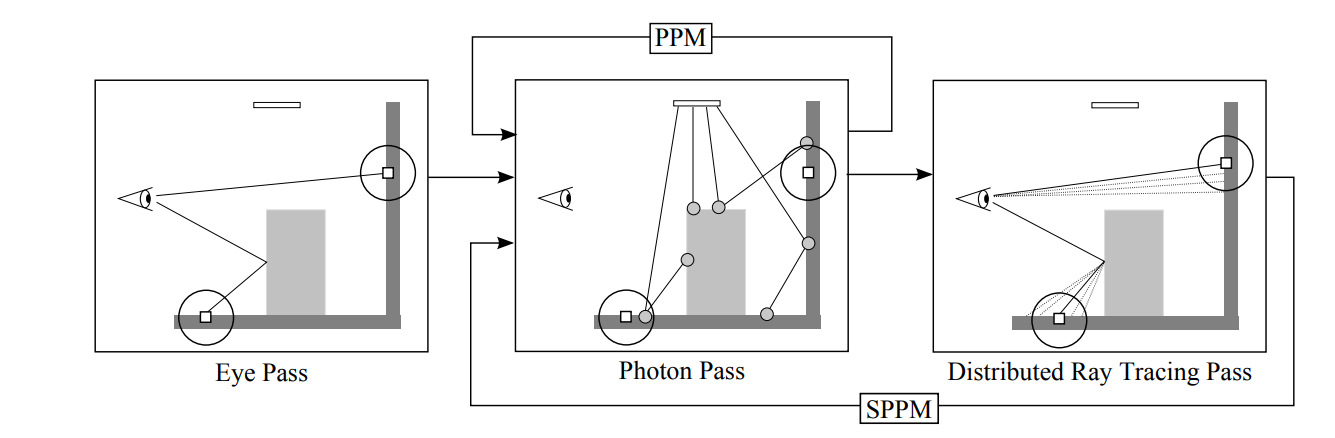
\includegraphics[scale=0.18]{Images/sppm.png}
			\caption{SPPM pipeline}\label{}
			\end{figure}
		As the above figure shows, we do one distributed ray tracing pass and one photon pass each round. The basic pipeline is shown as below.
		\begin{enumerate}
			\item [1.] Prepare for rendering. Set sample per pixel $spp$, number of photons $ptn\_num$, initial search radius $init_r$, 
			attenuation coefficient $\alpha$, total render round $rnd\_num$ and initial photon energy $e = \frac{1 - \alpha}{1 - \alpha^{rnd\_num}}$
			\item [2.] Reset viewpoints and temporary pixel energy, make sure they are clear before ray tracing pass.
			\item [3.] In every pixel, we shoot number of $spp$ rays randomly, and then do Ray tracing pass to get the viewpoints.
			\item [4.] Use the viewpoints we get from all pixels to construct a viewpoint KD-tree.
			\item [5.] We randomly generate $ptn\_num$ rays from light source, and do Photon tracing pass with current search radius $r$.
			\item [6.] We update the pixels color using temporary pixel energy calculated in photon tracing pass.
			\item [7.] Update search radius $r = r * \alpha$, update photon energy $e = e * \alpha$.
			\item [8.] If current render round > $rnd\_num$, stop rendering and output the image. Otherwise, go back to step2 to start next round.
		\end{enumerate}
		\subsection{Ray Tracing}
		Ray tracing is the first pass in both PPM and SPPM. 
		This part is not like path tracing but simpler.
		Each ray generated from the camera will stop right after hitting a diffuse surface.
		Only if the hit surface is not a diffuse one does it sample another ray to trace.

		After hitting a diffuse surface, the position will be stored as a viewpoint.
		Later in photon tracing part, the radiance of the viewpoint will be calculated,
		and the color will be set back to the corresponding pixel.

		Here the viewpoint are stored in a balanced KD-Tree for speed reason.
		The intersection part uses BVH for that triangles may intersect with different bounding boxes in KD-Tree which results in inefficiency.

	\subsection{Photon Tracing}
		In standard photon mapping method, photons are stored and each viewpoint needs to find all photons within a radius.
		Here we implemented SPPM, where we stored the viewpoints and let the photons find the nearby viewpoints instead. 
		This modification costs less memory when the photon number is large. 

		In each render iteration, we shoot a certain number of rays from the light, 
		each ray sampled according to the light distribution representing the path of a photon. 
		If a photon hits an ideal diffuse surface, the view points within a certain radius from the hitting point will be illuminated, 
		and the color of the corresponding pixels will be updated according to the viewpoint color from the object and the photon radiance. 
		Whenever a photon hits a geometry surface, a new ray will be sampled according to the brdf of the surface, 
		and the photon radiance will update by multiplying the brdf value. Here's the rendering equation:
		\begin{align}
			L(S,\omega) = \lim_{i \to \infty} \frac{\tau _i (S,\omega)}{N_e(i)\pi R_i(S)^2}
		\end{align}	where $N_e(i)$ is the photon number, $R_i(S)$ is the radius and $\tau _i (S,\omega)$ represents the total radiance, where
		
		\begin{align}
			\tau _i (S,\omega) = \sum_{p = 1}^{N(x)} f_r(x,\omega, \omega_p)\Phi_p(x_p,\omega_p)
		\end{align}
		And the new photon energy is combined with the brdf:
		\begin{align}
			\Phi_{p}^{'} = \Phi_p  f_r
		\end{align}
		For every photon, we apply the algorithm above.

	\subsection{Contribution}
	Member 1. Chunhao Bi  : \ Ray tracing and Path tracing, Materials and Texture, Algorithm Corrections.\\ 
	Member 2. Hongdi Yang : \ Rendering pipeline, Light settings, Scene construction.\\
	Member 3. Mutian Li   : \ Photon tracing, Color calculation

\section{Experiments}
	\subsection{Radius}
	This algorithm can render realistic pictures only if the initial radius is within an appropriate range. 
	If the radius is too large, some occluded area will be illuminated, and some shadow will disappear. 
	If the radius is too small and the number of photons is insufficient, the output image will be noisy on account of bright areas around the photons, 
	and this problem can be solved by increasing the number of photons. 
	Generally, decreasing the initial radius and increasing the number of photons simultaneously will render a more realistic image. 
	Fig.2. shows the render results with different initial radius, when the number of photons is 10000, with $spp = 1$, total render round = 10, attenuation coefficient $\alpha = 0.8$, search depth $depth = 8$.
	\begin{figure}[H]
	\centering
	\subfigure[radius=1]{
		\begin{minipage}[t]{0.45\linewidth}
		\centering
		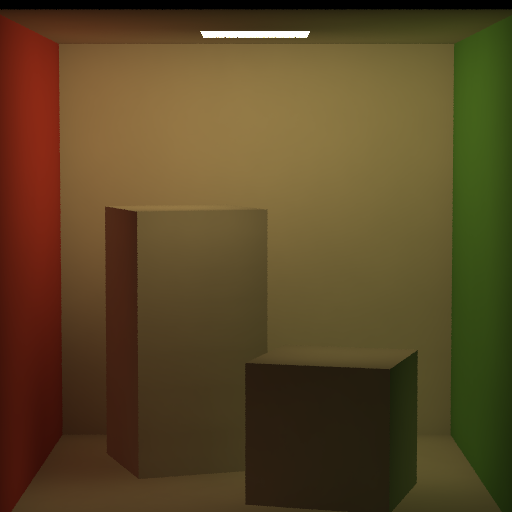
\includegraphics[width=1.5in]{Images/radius1.png}
		
		\end{minipage}%
		}
	\subfigure[radius=0.5]{
		\begin{minipage}[t]{0.45\linewidth}
		\centering
		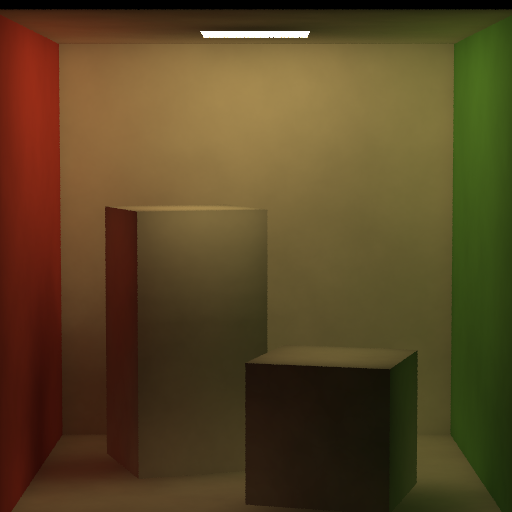
\includegraphics[width=1.5in]{Images/radius0.5.png}
		
		\end{minipage}%
		}
	\subfigure[radius=0.25]{
		\begin{minipage}[t]{0.45\linewidth}
		\centering
		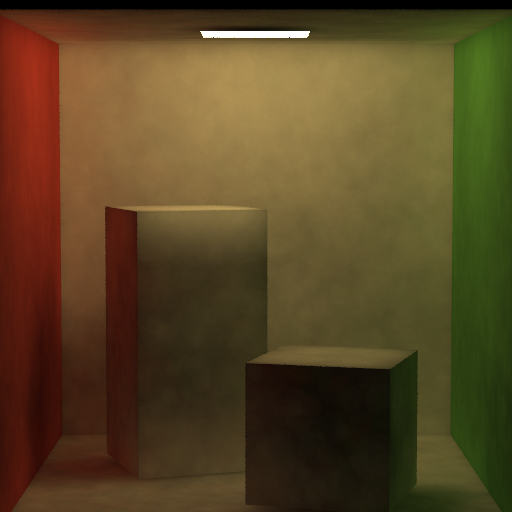
\includegraphics[width=1.5in]{Images/radius0.25.png}
		
		\end{minipage}%
		}
	\subfigure[radius=0.125]{
		\begin{minipage}[t]{0.45\linewidth}
		\centering
		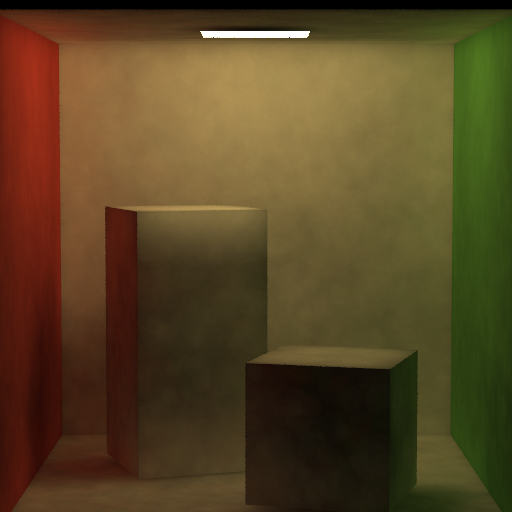
\includegraphics[width=1.5in]{Images/radius0.25.png}
		
		\end{minipage}%
		}
		\caption{Radius}
	\end{figure} 
	A smaller update coefficients will accelerate the convergence, and the image will be more realistic under the same number of total render rounds, 
	but might become noisy during the last several rounds, and the reason is the same as a small radius. 
	Therefore, increasing the number of photon will overcome the unexpected noise. The following figure shows the results with different attenuation coefficients, 
	when the number of photons is 10000, with $spp = 1$, total render round = 10, initial search radius $r = 0.5$, search depth $depth = 8$.
	\begin{figure}[H]
	\centering
	\subfigure[coefficient=0.8]{
		\begin{minipage}[t]{0.3\linewidth}
		\centering
		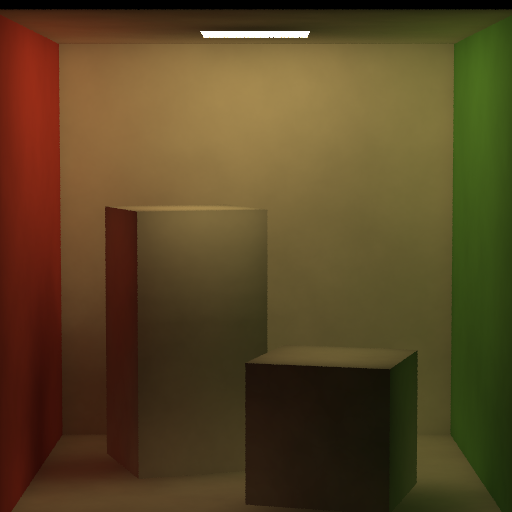
\includegraphics[width=1in]{Images/radius0.5.png}
		
		\end{minipage}%
		}
	\subfigure[coefficient=0.7]{
		\begin{minipage}[t]{0.3\linewidth}
		\centering
		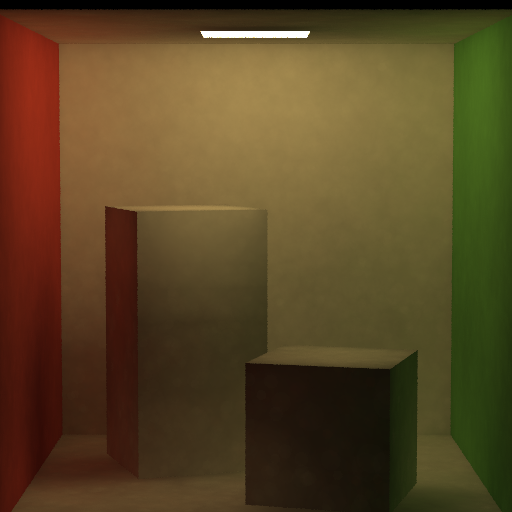
\includegraphics[width=1in]{Images/decay0.7.png}
		
		\end{minipage}%
		}
	\subfigure[coefficient=0.5]{
		\begin{minipage}[t]{0.3\linewidth}
		\centering
		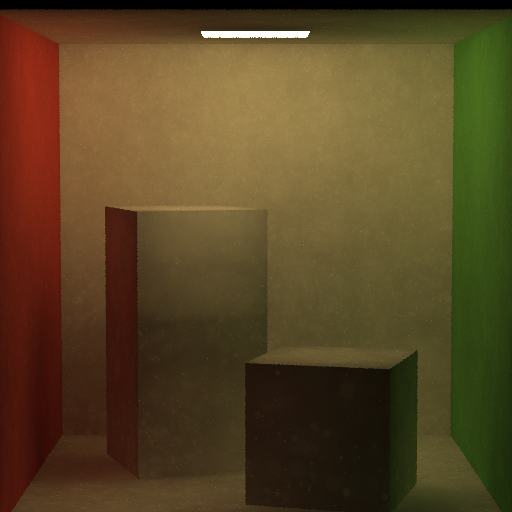
\includegraphics[width=1in]{Images/decay0.5.png}
		
		\end{minipage}%
		}
		\caption{Attenuation coefficient}
	\end{figure} 
	
	\subsection{Round number}
	Here we show how our render result progress with render round increases.
	\begin{figure}[H]
		\centering

		\subfigure[Render round 0]{
		\begin{minipage}[t]{0.45\linewidth}
		\centering
		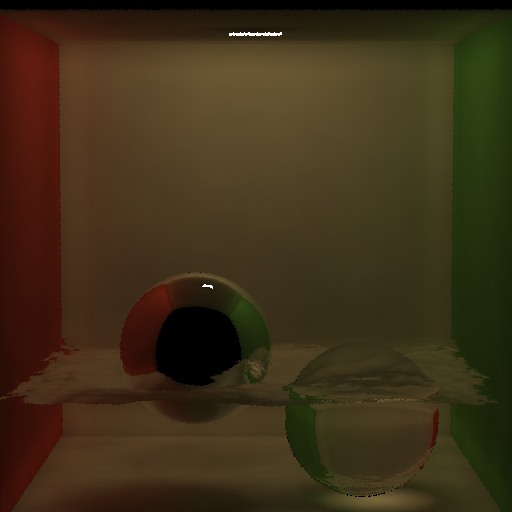
\includegraphics[width=1.5in]{Images/Water_round20_photon200000_r0.15_alpha0.8/output_round0.png}
		%\caption{original image}
		\end{minipage}%
		}
		\subfigure[Render round 4]{
		\begin{minipage}[t]{0.45\linewidth}
		\centering
		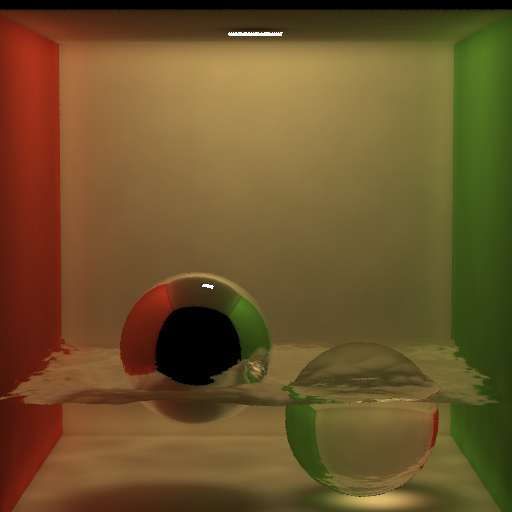
\includegraphics[width=1.5in]{Images/Water_round20_photon200000_r0.15_alpha0.8/output_round4.png}
		%\caption{ground truth}
		\end{minipage}%
		}%

		\subfigure[Render round 9]{
			\begin{minipage}[t]{0.45\linewidth}
			\centering
			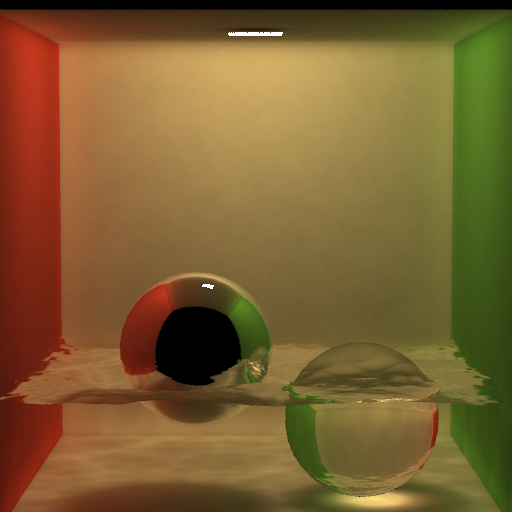
\includegraphics[width=1.5in]{Images/Water_round20_photon200000_r0.15_alpha0.8/output_round9.png}
			%\caption{original image}
			\end{minipage}%
			}
			\subfigure[Render round 14]{
			\begin{minipage}[t]{0.45\linewidth}
			\centering
			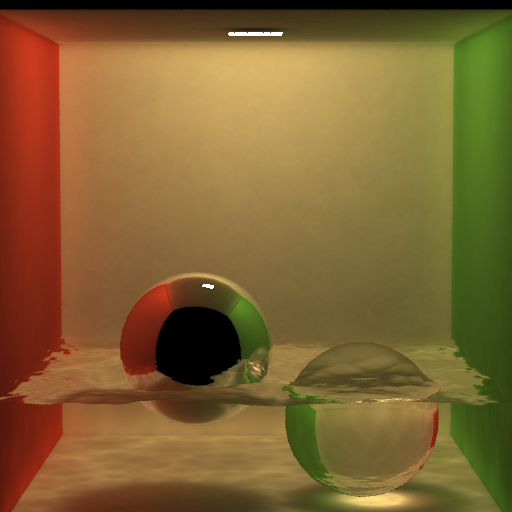
\includegraphics[width=1.5in]{Images/Water_round20_photon200000_r0.15_alpha0.8/output_round14.png}
			%\caption{ground truth}
			\end{minipage}%
			}%

			\subfigure[Render round 19]{
				\begin{minipage}[t]{0.45\linewidth}
				\centering
				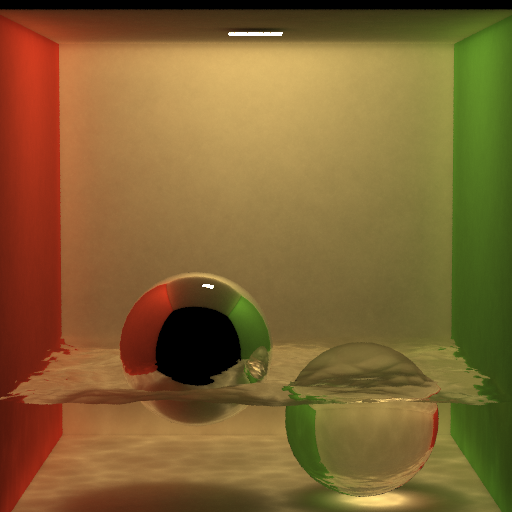
\includegraphics[width=1.5in]{Images/Water_round20_photon200000_r0.15_alpha0.8/output_round19.png}
				%\caption{ground truth}
				\end{minipage}%
				}%
				\caption{Render results}
	\end{figure}
	As Figure2 shows, as render round increases, our render result gets brighter and more realistic. 
	As we decrease the search radius every round, the calculated radiance will converge to the real radiance. 
	And this will be quite efficient for caustics effect as there will be many rays hitting a relatively small area through translucent objects.
	\begin{figure}[H]
		\centering
		
		\subfigure[Round 0]{
		\begin{minipage}[t]{0.18\linewidth}
		\centering
		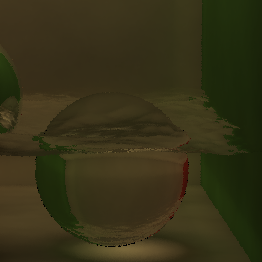
\includegraphics[width=.5in]{Images/caustics0.png}
		%\caption{original image}
		\end{minipage}%
		}
		\subfigure[Round 4]{
		\begin{minipage}[t]{0.18\linewidth}
		\centering
		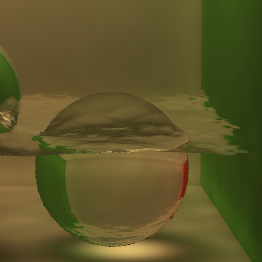
\includegraphics[width=0.5in]{Images/caustics4.png}
		%\caption{ground truth}
		\end{minipage}%
		}%
		\subfigure[Round 9]{
		\begin{minipage}[t]{0.18\linewidth}
		\centering
		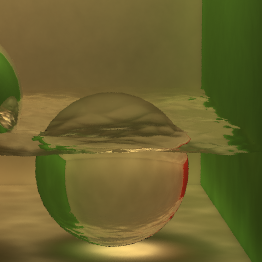
\includegraphics[width=0.5in]{Images/caustics9.png}
		%\caption{original image}
		\end{minipage}%
		}
		\subfigure[Round 14]{
		\begin{minipage}[t]{0.18\linewidth}
		\centering
		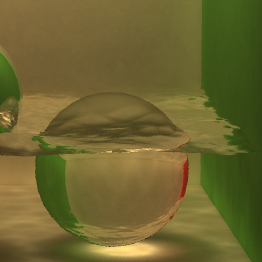
\includegraphics[width=0.5in]{Images/caustics14.png}
		%\caption{ground truth}
		\end{minipage}%
		}%
		\subfigure[Round 19]{
		\begin{minipage}[t]{0.18\linewidth}
		\centering
		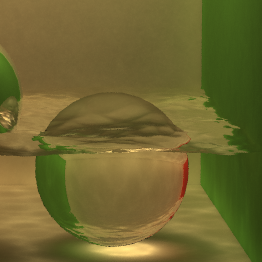
\includegraphics[width=0.5in]{Images/caustics19.png}
		%\caption{ground truth}
		\end{minipage}%
		}%
		\caption{caustics effects}
	\end{figure} 
	As Figure3 shows, the caustics effect become much better as the render round increases.
	
	
	Also, as search radius decreases, there will be fewer photons found around each viewpoint, thus making the render time faster.
	Under the parameter of : $spp = 1$, photon number = 200000, initial search radius $r = 0.15$, total render round = 20, attenuation coefficient $\alpha = 0.8$,
	search depth $depth = 32$, we record the time for some render rounds.
	\begin{figure}[H]
		\centering
		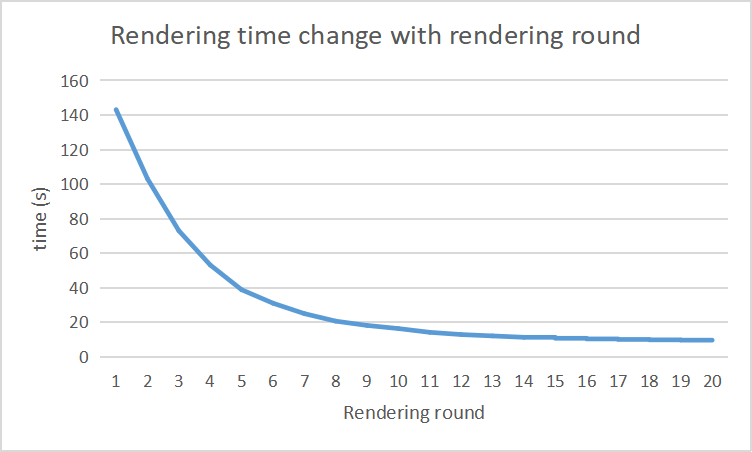
\includegraphics[scale=0.5]{Images/render_round.png}
		\caption{Rendering time change with rendering round}\label{}
		\end{figure}
	\subsection{Comparison}
	Comparison between different render methods is important.
	For photon mapping method, if the parameters are set well, the converging speed will be much higher comparing to basic path tracing method.


	We tried rendering the same scene with Monte-carlo ray tracing and our method. In ray tracing, the parameters are : $spp$ = 256,
	search depth = 8. In photon mapping, the parameters are : $spp = 1$, photon number = 200000, initial search radius $r = 0.15$, total render round = 20, attenuation coefficient $\alpha = 0.8$,
	search depth $depth = 8$. Here are the results.
	\begin{figure}[H]
		\centering
		
		\subfigure[Monte-carlo]{
		\begin{minipage}[t]{0.4\linewidth}
		\centering
		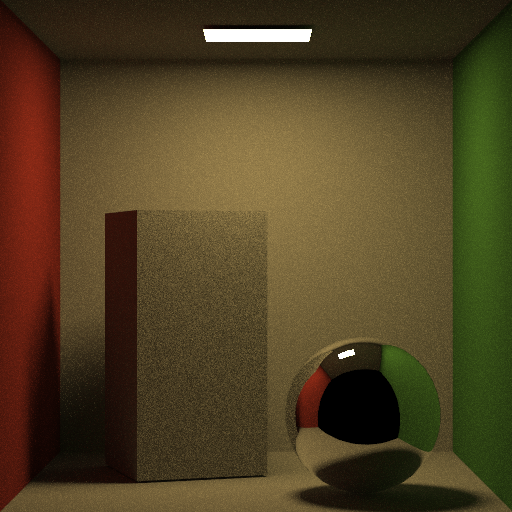
\includegraphics[width=1.2in]{Images/ray_tracing.png}
		%\caption{original image}
		\end{minipage}%
		} \
		\subfigure[SPPM]{
		\begin{minipage}[t]{0.4\linewidth}
		\centering
		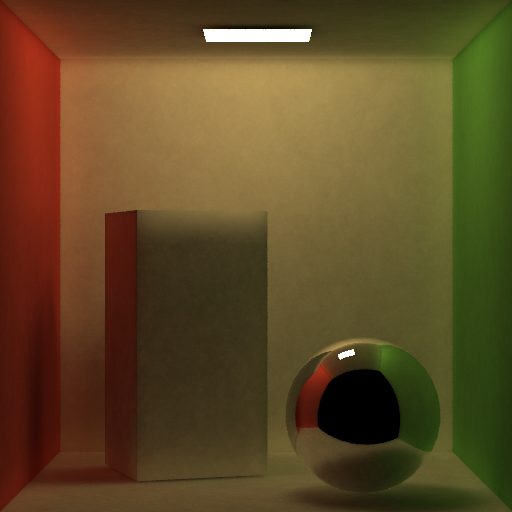
\includegraphics[width=1.2in]{Images/sppm_result.png}
		%\caption{ground truth}
		\end{minipage}%
		}%
	\end{figure}
	For Monte-Carlo ray tracing, it takes 1313s to render. For photon mapping, it only takes 502s. 


	There are some metrics in path tracing, which use different method to make it converge faster, such as direct light sampling, bidirectional sampling and metropolis sampling.
	However, those methods are still quite slow for that they are still sampling pixels.
	Photon mapping changes the rule, which makes it possible for some scenes with severe light condition.
	Here we compared the results of naive path tracing, path tracing with direct light sampling, and SPPM with the same rendering time of about 550000ms.
	\begin{figure}[H]
		\centering
		
		\subfigure[Monte-carlo]{
		\begin{minipage}[t]{0.32\linewidth}
		\centering
		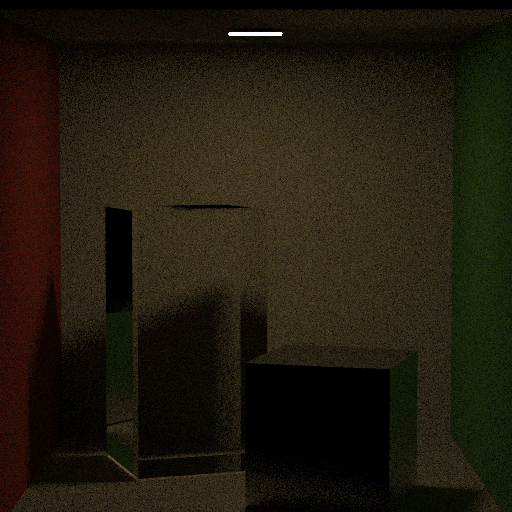
\includegraphics[width=1in]{Images/comparision/monte carlo.png}
		%\caption{original image}
		\end{minipage}%
		}
		\subfigure[Direct light sampling]{
		\begin{minipage}[t]{0.32\linewidth}
		\centering
		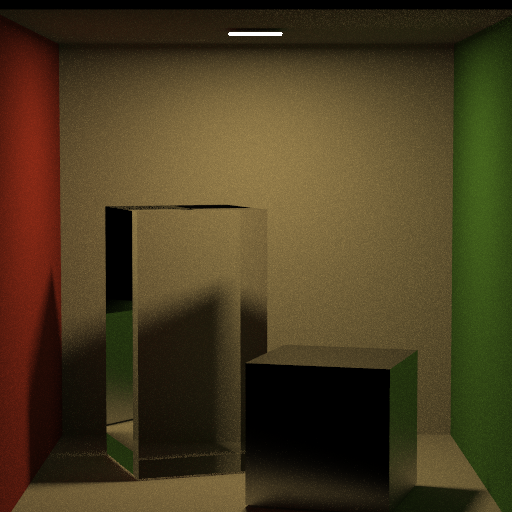
\includegraphics[width=1in]{Images/comparision/direct lighting.png}
		%\caption{ground truth}
		\end{minipage}%
		}%
		\subfigure[SPPM]{
		\begin{minipage}[t]{0.32\linewidth}
		\centering
		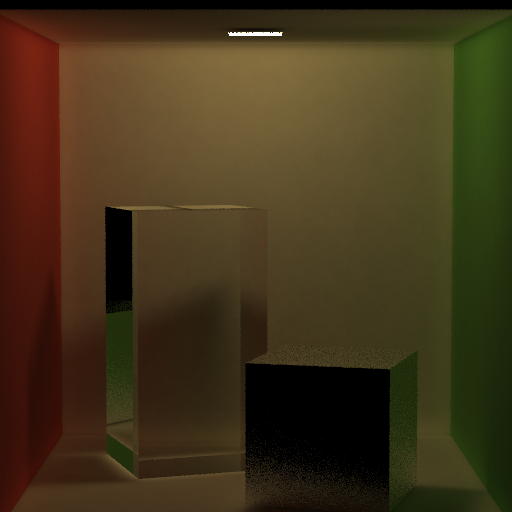
\includegraphics[width=1in]{Images/comparision/500000ms/output.png}
		%\caption{original image}
		\end{minipage}%
		}
		\caption{Same scene rendered by different methods}
	\end{figure} 
	From the figure above, the naive method converges really slow because of the small light source to reach.
	The direct light sampling method does quite good on the walls, but because the translucent boxes are considered light-tight,
	the shadow area converges as slow as using naive method. 
	This converging speed difference results in misleading understanding of the scene.
	The SPPM method gets a good result for the scene with the translucent part. 
	The shadow of the long box is quite soft which representing a far more converged result.
	However, the result seem not so good at glossy materials telling from the noise on the short box compared to direct light sampling.

\section{Results}
Here are some of our final render results.

Parameters: $spp = 1$, photon number = 200000, initial search radius $r = 0.15$, total render round = 20, attenuation coefficient $\alpha = 0.8$,
search depth $depth = 32$
\begin{figure}[h]
	\centering
	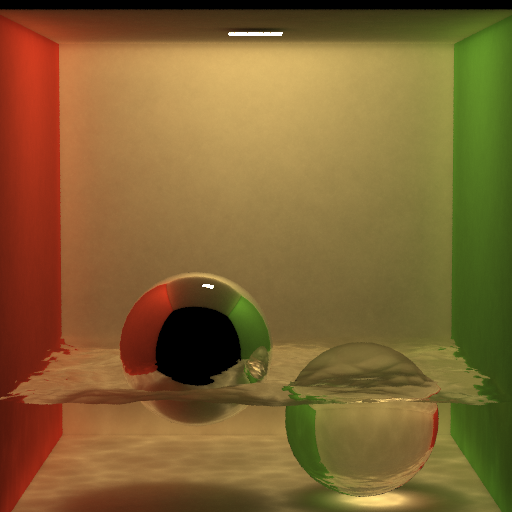
\includegraphics[scale=0.3]{Images/Water_round20_photon200000_r0.15_alpha0.8/output_water.png}
	\caption{Scene with Water and spheres}
	\end{figure}
\begin{figure}[h]
		\centering
		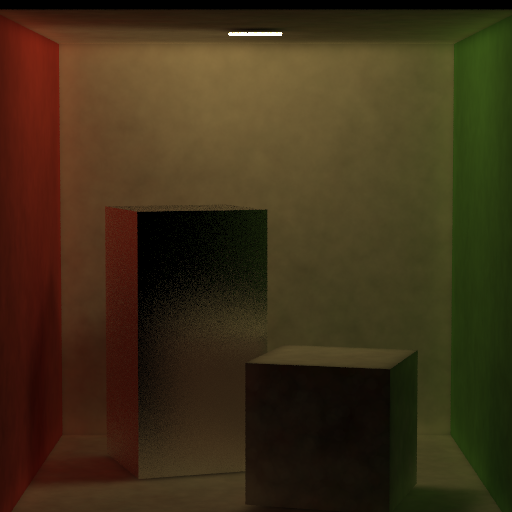
\includegraphics[scale=0.3]{Images/glossy.png}
		\caption{Cube with glossy surface}
	\end{figure}
\begin{figure}[h]
		\centering
		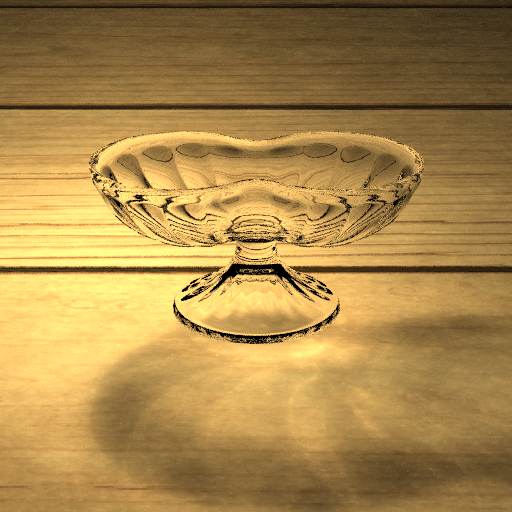
\includegraphics[scale=0.3]{Images/icecream.png}
		\caption{An ice-cream bowl made of glass}
	\end{figure}
	\begin{figure}[h]
		\centering
		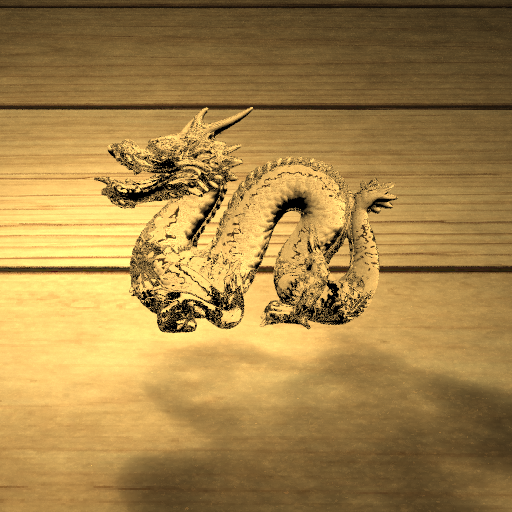
\includegraphics[scale=0.3]{Images/dragon.png}
		\caption{Dragon made of glass}
	\end{figure}	
	\begin{figure}[h]
		\centering
		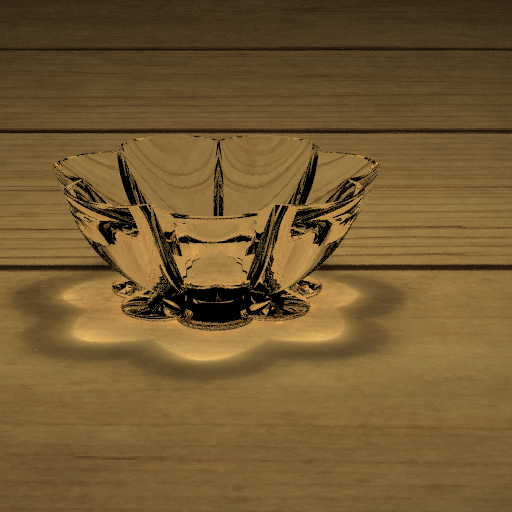
\includegraphics[scale=0.3]{Images/output_20round_photon500000.png}
		\caption{A flower pot made of glass}
	\end{figure}		
	\begin{figure}[h]
		\centering
		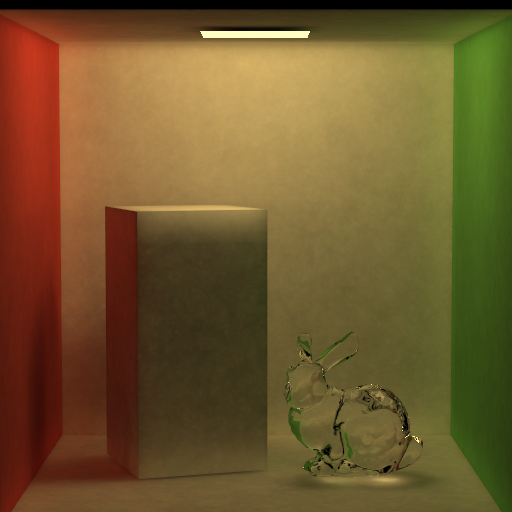
\includegraphics[scale=0.3]{Images/output_spp10.png}
		\caption{diffuse cube and translucent bunny}
	\end{figure}
	\begin{figure}[h]
		\centering
		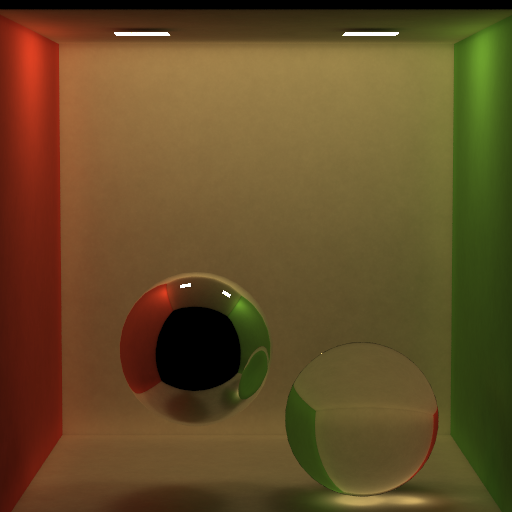
\includegraphics[scale=0.3]{Images/multiple_lights.png}
		\caption{Scene under multiple lights}
	\end{figure}
	\begin{figure}[h]
		\centering
		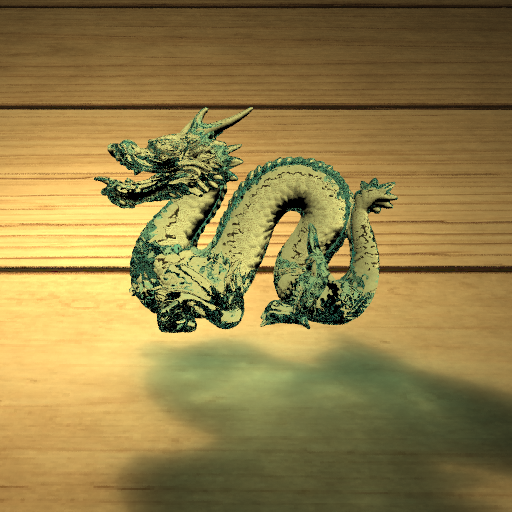
\includegraphics[scale=0.3]{Images/icedragon.png}
		\caption{Ice dragon}
	\end{figure}
	\end{document}
